% -*- TeX-master: "master" -*-

\section{Experiments}
\label{sec-experiments}

This section presents quantitative data about the ideas presented in previous sections.  This data was collected using the Siemens test suite \cite{257766} as maintained by the Galileo Software-artifact Infrastructure Repository (SIR) \cite{Do05,SAI}.  There are two configurable parameters for the experiments: the sampling rate and the $\effort$ cutoff (described in \autoref{sec-metrics}).  Unless specified, the default sampling rate is 1 (i.e., complete data collection) and the default $\effort$ is 5\% (only predicates that are reachable from each other by exploring less than 5\% of the program are considered).  Each Siemens application is available in multiple variants with different bugs: as few as 9 variants of \prog{schedule2} and as many as 41 variants of \prog{tcas}.  We report aggregate results by averaging the relevant measures across all variants of each Siemens application.

\subsection{Top Scoring Predicates}

\label{sec-quant}
\begin{figure}[tb]
  \centering
  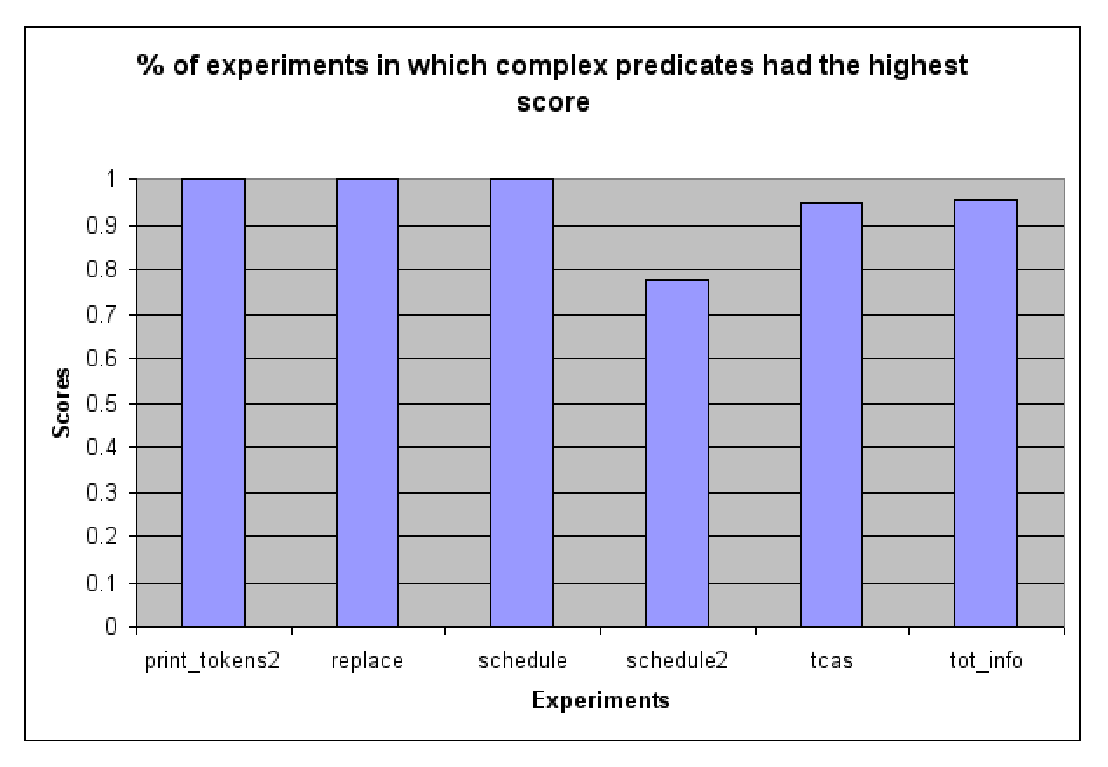
\includegraphics{charts/top-pred}
  \caption{Fraction of buggy application variants having a complex predicate as the top-scoring predictor}
  \label{fig-top-pred}
\end{figure}

\autoref{fig-top-pred} plots the percentage of variants within each program for which a complex predicate had the highest score among all predicates.  The value is 100\% for \prog{print\_tokens}, \prog{print\_tokens2} and \prog{schedule} and is close to 100\% for the other programs.  The results shown in \autoref{fig-top-pred} combined with the case studies in \autoref{sec-qual} show that program behavior can be accurately predicted using constructed predicates.

\subsection{Effectiveness of Pruning}
\label{sec-effectprune}
\begin{figure*}[tb]
  \centering
  \subfloat[Conjunctions]{\includegraphics{charts/pruning-conj}}
  \hfill
  \subfloat[Disjunctions]{\includegraphics{charts/pruning-disj}}
  \caption{Avoiding computing exact scores by pruning complex predicates.  ``Overall'' summarizes the entire Siemens suite.}
  \label{fig-pruning}
\end{figure*}

Even when restricted to binary conjunction and disjunction, complex predicates could substantially increase the analysis workload if na\"ively implemented.  \autoref{sec-metrics} suggests heuristics for pruning complex predicates that are unlikely to be useful or understandable to a programmer, while \autoref{sec-pruning} describes how to compute an upper bound on a predicate's score.  \autoref{fig-pruning} shows that these measures are highly effective in practice.  On average, 53\% of candidate complex predicates are discarded because the $\effort$ as defined in \autoref{def-effort} would require traversing more than 5\% of the application code. Computing the exact scores of the remaining 47\% of the complex predicates takes, on average, 9 minutes.  Pruning complex predicates whose upper bound of the $\Importance$ scores, computed per \autoref{sec-pruning}, are lower than the scores of their constituent simple predicates eliminates a further 25\% of the complex predicates.  This pruning reduced the average time required per analysis to 6 minutes.  An aggressive application of this pruning by including the score of the top simple predicate as the threshold reduced the average time taken to a minute.  Only 22\% of complex predicates remain to have their exact scores computed, of which roughly a fourth (6\% of the initial pool) are retained as potentially interesting bug predictors.  Thus we find that the techniques proposed earlier significantly reduce the computational load required to identify a useful, high-scoring subset of complex predicates.


\subsection{Effect of Effort}

\begin{figure*}[tb]
  \centering
  \subfloat[Conjunctions]{\includegraphics{charts/effort-conj}}
  \hfill
  \subfloat[Disjunctions]{\includegraphics{charts/effort-disj}}
  \caption{Variation of number of interesting predicates with $\effort$}
  \label{fig-effort}
\end{figure*}

\autoref{fig-effort} shows how the number of interesting conjunction and disjunction predicates (\autoref{dfn3}) varies at four different $\effort$ levels.  As expected, as $\effort$ increases more predicates are evaluated and so more interesting predicates are found.

\subsection{Effect of Sampling Rate}
\label{sec-sampling}

Real deployments of CBI use sparse random sampling of simple
predicates to reduce performance overhead and protect user privacy.
Prior work \cite{Liblit:2003:BIRPS} has recommended sampling rates of
\nicefrac{1}{100} to \nicefrac{1}{1000} to balance data quality
against performance and privacy concerns.  However, a pair of
independent features each observed in \nicefrac{1}{100} runs have only
a \nicefrac{1}{10,000} chance of being observed together, raising
doubts whether interesting complex predicates will be found in
sparsely sampled data.

\begin{table*}[tb]
  \centering
  \begin{tabular}{lrrrrrrrrr}
    \toprule
    & \multicolumn{3}{c}{Simple}
    & \multicolumn{3}{c}{Conjunctions}
    & \multicolumn{3}{c}{Disjunctions}
    \\
    \cmidrule(r){2-4} \cmidrule(lr){5-7} \cmidrule(l){8-10}
    Application
    & \nicefrac{1}{1} & \nicefrac{1}{100} & \nicefrac{1}{1,000}
    & \nicefrac{1}{1} & \nicefrac{1}{100} & \nicefrac{1}{1,000}
    & \nicefrac{1}{1} & \nicefrac{1}{100} & \nicefrac{1}{1,000}
    \\
    \midrule
    \input{charts/sampling-rows}
    \bottomrule
  \end{tabular}
  \caption{Sampling rate vs. number of interesting predicates,
    averaged across all variants of each Siemens application. ``-'' marks
    an average count of exactly zero, i.e., no interesting predicates in
    any variant.}
  \label{tab-sampling}
\end{table*}

\begin{figure}[tb]
  \centering
  \includegraphics{charts/sampling-print_tokens2}
  \caption{Sampling rate vs. number of interesting predicates,
    averaged across all variants of \prog{print\_tokens2}.  Other
    Siemens applications are similar.}
  \label{fig-sampling}
\end{figure}

\autoref{tab-sampling} shows the average number of interesting simple
and complex predicates found is each Siemens application for both
complete data collection (\nicefrac{1}{1}) and two realistic sampling
rates.  \autoref{fig-sampling} shows the same information at
additional, denser rates for \prog{print\_tokens2}.  Other Siemens
applications behave similarly and are omitted for brevity.

The number of interesting disjunctions is always very low (order of
tens) compared to interesting conjunctions.  At sampling rates lower
than \nicefrac{1}{10}, there is a sharp drop in the number of
interesting conjunctions.  This is likely due to the shrinking odds of
observing both components of a conjunction within a single run.
Despite the sharp drop, the number of interesting conjunctions is
still comparable to the number of interesting simple predicates even
at \nicefrac{1}{1000} sampling.  This shows that interesting complex
predicates can still be found at sparse but realistic sampling rates.

A puzzling trend in \autoref{fig-sampling} is that all three curves
rise for a brief interval before dropping off.  Other Siemens
applications exhibit a similar bump.  The bumps in the conjunction and
disjunction curves could be attributed to the bump in the simple
predicates curve.  Any increase in the number of interesting simple
predicates is likely to produce a greater increase in the number of
interesting complex predicates, especially because the additional
simple predicates are likely to be redundant (as explained later).

The transient increase in the number simple predicates at moderate
sampling rates was previously undiscovered and initially seems
counterintuitive.  Closer inspection of experimental results reveals
two scenarios where this can happen.

The first scenario happens due to an ad hoc, but perfectly reasonable
elimination of seemingly identical predicates.  As an example, consider the
predicates $p$: \texttt{a == b} and $q$: \texttt{a >= b}.  If they have the
same score, it is useful to just retain $p$ as it is a more stringent
condition than $q$.  However, this does not mean
that \texttt{a > b} was never true.  \texttt{a > b} may be observed  during 
some runs but does not affect the outcome of \texttt{a >= b} if \texttt{a == b}
also happens to be true in those runs.  However, at sampling rates lower than
1, only \texttt{a > b} may be observed in some runs and hence the number of
runs in which $p$ and $q$ are observed \emph{true}, and consequently their
scores may be different.  Thus, the ad hoc elimination heuristic performs 
less effectively at lower sampling rates, leading to an increase in the 
number of interesting simple predicates

To understand the second scenario, consider a predicate $p$ for which
$\obs{S}{p} = S(p)$ and $\obs{F}{p} = F(p)$.
In other words, $p$ is true at least once in every run in which it is
observed.  From \autoref{eqn1}, $\Increase(p) = 0$.  In a run 
in which $p$ was observed, it may also be \emph{false} atleast once.  As we
reduce the sampling rates, only the \emph{false} occurences may be recorded
in some runs and hence the two equalities may no longer hold.  As a result
$\Increase(p)$ may be nonzero and if it becomes positive a predicate that
was not interesting at higher sampling rates becomes interesting at lower 
sampling rates.
